\documentclass{beamer}
\usepackage{Freifunkstil}
\begin{document}
\title[Freifunk]{Freifunk - Was ist das?}
\subtitle[Offene Netze]{Wir bauen gemeinsam freie Netze.}
\author{MikeTsenatek \& b3yond}
\date{\today\\\vspace{0.5cm} 
\includegraphics[scale=0.3]{images/logo-transparent.png}}
\institute{Freifunk Franken}

\begin{frame}
\titlepage	
\end{frame}
\begin{frame}{Inhaltsverzeichnis}
	\tableofcontents
\end{frame}


\section{Allgemein}
\begin{frame}
\begin{itemize}
\item Test
\item Test2
\end{itemize}
\end{frame}

\section{Technik}


\subsection{Test1}
\begin{frame}


tesst


dsfdsf


dsf


dsf



sdf

\begin{itemize}
\item Test
\item Test2
\end{itemize}
\end{frame}


\subsection{Test2}
\begin{frame}

\begin{itemize}
\item Test
\item Test2
\end{itemize}
\end{frame}
\section{Die Community}

\begin{frame}
\frametitle{Status Deutschland}
	\begin{columns}[c]   
		\begin{column}[T]{0.6\textwidth}     
			\begin{itemize}
				\item ca. 280 Communities \footnotemark[1]
				\item ca. 30.000 Access Points \footnotemark[1]
				\item Offizl. Staatliche Unterstützung:
				\begin{itemize}
					\item Pfalz, Sachsen-Anhalt, Nordrhein-Westfalen 
				\end{itemize}
				\item Offizl. Städtische Unterstützung:
				\begin{itemize}
					\item Berlin, Dresden, Magdeburg, Arnsberg, Osnabrück, Bochum, Mainz, München, Erlangen usw...
				\end{itemize}
			\end{itemize}
		\end{column}
		\begin{column}[T]{0.4\textwidth}     
			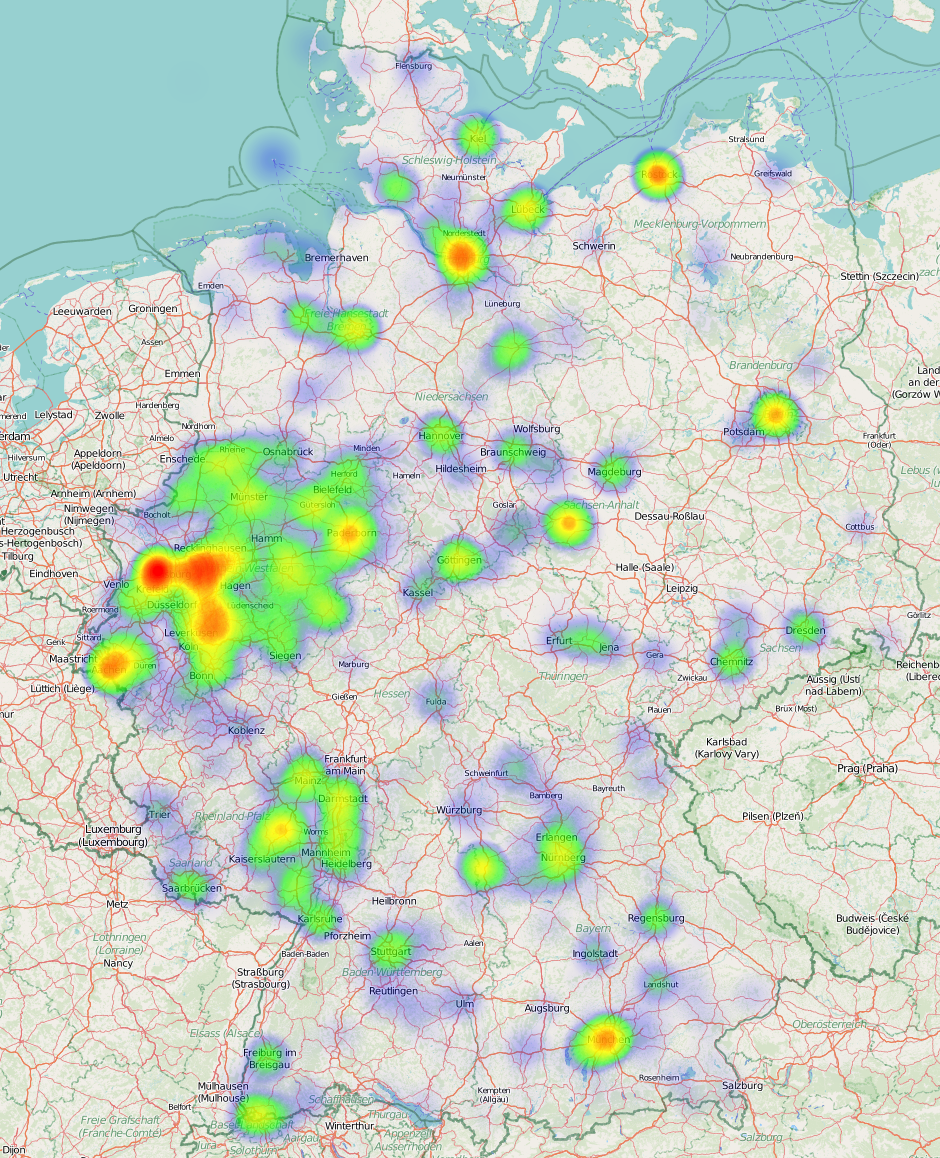
\includegraphics[width=\textwidth]{images/heatmap_germany.png} 
		\end{column}
	\end{columns}		
	\footnotetext[1]{Stand: 12.03.2016}

\end{frame}





\end{document}
